\documentclass[11pt]{article}

\usepackage[T1]{fontenc}
\usepackage{lmodern}
\usepackage[margin=1in]{geometry}
\usepackage{microtype}
\usepackage{amsmath,amssymb}
\usepackage{booktabs}
\usepackage{array}
\usepackage{tabularx}
\usepackage{graphicx}
\usepackage{xcolor}
\usepackage[round,authoryear]{natbib}
\usepackage[font=small,labelfont=bf]{caption}
\usepackage[colorlinks=true,allcolors=blue!55!black]{hyperref}
\usepackage{xurl}

\graphicspath{{figures/}{../reports/figures/}}

\definecolor{navy}{HTML}{183B56}
\definecolor{teal}{HTML}{147D92}
\definecolor{pale}{HTML}{F2F7F8}
\definecolor{warm}{HTML}{9A5B13}
\definecolor{softgray}{HTML}{666666}

\hypersetup{
  pdftitle={Partial cross-location generalization of a CA1 wall-related population contrast},
  pdfauthor={Javier Emilio Bazan Sanchez},
  pdfsubject={Longitudinal CA1 population coding}
}

\newcommand{\meanrho}{\overline{\rho}}
\newcommand{\R}{\mathbb{R}}
\newcommand{\stepbox}[2]{%
  \fcolorbox{teal}{pale}{%
    \parbox[c][2.15cm][c]{0.205\textwidth}{%
      \centering\small\textbf{\color{navy}#1}\par\vspace{0.45em}#2}}}

\title{\textbf{Partial cross-location generalization of a CA1 wall-related population contrast}\\
\large An exploratory longitudinal reanalysis}
\author{Javier Emilio Bazan Sanchez\\
\small Facultad de Ciencias, Universidad Nacional Aut\'onoma de M\'exico
(UNAM)\\
\small\href{mailto:bazan@ciencias.unam.mx}{bazan@ciencias.unam.mx}}
\date{Working manuscript -- August 1, 2026}

\begin{document}
\maketitle

\begin{abstract}
Environmental boundaries strongly influence hippocampal place fields, but it
is unresolved whether wall-related remapping generalizes across physical
locations. We reanalysed longitudinal calcium-imaging data from 5,413 dorsal
CA1 neurons in seven mice across repeated exposure cycles containing a familiar
square and nine internal-wall geometries. A cell-resolved wall-minus-open
contrast estimated at one location predicted later held-out responses at the
same location (mean correlation advantage $0.184$; seven of seven animals). A
single-tile counterfactual gave the same result ($0.225$; seven of seven),
including after adjustment for speed, heading, time, occupancy, and spatial
sampling. Crucially, a contrast estimated at a non-overlapping source seam
predicted a later wall response at a target seam 25 cm away
($\meanrho=0.148$; seven of seven animals) and remained positive after
behavioral adjustment ($\meanrho=0.119$). Cross-location prediction was weaker
than a query-matched exact-location benchmark ($\meanrho=0.230$;
shifted-minus-exact $=-0.082$), demonstrating partial rather than complete
generalization. The correctly oriented source also exceeded an empirical
equal-midpoint wrong-orientation control by $0.101$ in all seven animals. A
strict same-session reflected-open control favored the wall target by $0.114$
in all five eligible animals, although raw-rate and fully distance-stratified
comparisons were less consistent. Thus a CA1 wall-related population contrast
generalizes beyond its original coordinate while retaining strong spatial
dependence. The exploratory, fixed-order design does not identify whether this
phenomenon reflects a wall-specific mechanism or more general spatial
deformation.
\end{abstract}

\noindent\textbf{Keywords:} hippocampus; CA1; place cells; boundaries;
population code; transfer; remapping; cognitive map

\section*{Significance statement}

We tested whether a cell-by-cell CA1 response contrast associated with a wall
at one location predicts a later wall response somewhere else. It did so in
all seven animals, including after behavioral adjustment, but less strongly
than at the original location. Spatial controls support relative wall
specificity while leaving some contribution from smooth place-field structure
unresolved. The central result is therefore a graded form of generalization:
hippocampal remapping is neither independent across locations nor fully
location invariant.

\section{Introduction}

Place cells relate an animal's position to a distributed hippocampal activity
pattern, yet the map is not a passive image of Euclidean space. Place fields
are anchored by environmental geometry, shift when boundaries move, and can
appear at characteristic distances and directions from walls
\citep{OKeefeBurgess1996,HartleyEtAl2000,BarryEtAl2006}. Boundary-responsive
inputs provide one mechanistic route by which local geometry could organize
hippocampal representations \citep{LeverEtAl2009}. More generally, current
accounts treat hippocampal-entorhinal codes as structured representations
whose parts may be recombined or generalized across experiences
\citep{StachenfeldEtAl2017,WernleEtAl2018,BakermansEtAl2025}.

These observations leave an important distinction unresolved. A wall-related
response may recur at the same coordinate despite changes elsewhere in the
environment. That is \emph{exact-location reuse}: a local feature of an
otherwise changing map remains stable. A stronger possibility is
\emph{cross-location transfer}: the cell-resolved response contrast evoked by
a wall at one seam predicts the response to a wall at a different seam. This
second claim is not implied by ordinary place-field stability or by the
existence of boundary-vector-like firing. It requires an out-of-sample test of
whether the identities and signed response changes of individual cells carry
across spatial coordinates.

The magnitude of cross-location prediction distinguishes three empirical
possibilities. Transfer comparable to exact-location reuse would indicate weak
dependence on coordinate; attenuated transfer would indicate partial
generalization within a place-dependent code; and absent transfer would be
consistent with responses reconstructed independently at each location. These
possibilities can agree on mean rate maps while differing in the
cross-registered population structure.

The dataset of \citet{LeeEtAl2025} is unusually useful for separating these
possibilities. Seven mice were imaged longitudinally in dorsal CA1 while
foraging in a familiar square and in nine environments made by placing
internal walls on a common spatial lattice. Repeated exposure cycles provided
registered cells, recurring local seams, and later held-out sessions. The
design was not created for a transfer test, so the present work is exploratory
and constrained by fixed environment order. Its geometry nevertheless permits
three progressively stronger questions: does an estimated wall-open contrast
recur at the same seam across global contexts; does an especially clean
single-tile contrast recur; and does a contrast estimated at one seam predict a
wall response at a neighboring, non-overlapping seam?

We find affirmative answers to all three, with an important gradient.
Exact-location prediction is strongest and cross-location prediction is
smaller but positive in every animal. The contribution is a specific
population-level observation: a wall-related CA1 response contrast retains
predictive information after a change of spatial coordinate.

\section{Results}

\subsection{A held-out test of cell-resolved wall contrasts}

We represented each candidate wall location as an oriented seam between two
adjacent lattice tiles. For a registered cell, an environment, and a seam, we
estimated activity in a narrow local strip and subtracted the corresponding
estimate from a bracketing familiar-square session. This square residual
reduced stable place preference while retaining the environment-specific local
change.

Training geometries supplied two cell-wise profiles at each seam: a mean
residual when the seam was blocked by a wall and a mean residual when it was
open. Their difference was the estimated wall-related contrast. The neural outcome
from the later target geometry was never used to form that source contrast.
Prediction was scored by a rank correlation across held-out registered cells.
We report animal-level means and sign counts rather than treating cells or
queries as independent biological replicates.

\begin{figure}[t]
\centering
\begin{tabularx}{\linewidth}{@{}XcXcX@{}}
\stepbox{1. Estimate}{Other geometries identify wall and open responses at a
source seam.}
&
\raisebox{1.05cm}{$\boldsymbol{\longrightarrow}$}
&
\stepbox{2. Register}{The signed wall-minus-open contrast is retained for the
same cells.}
&
\raisebox{1.05cm}{$\boldsymbol{\longrightarrow}$}
&
\stepbox{3. Test}{Predict a later wall response at the exact seam or a
non-overlapping seam.}
\end{tabularx}
\vspace{0.8em}

\begin{tabularx}{0.94\linewidth}{@{}>{\centering\arraybackslash}X
  >{\centering\arraybackslash}X@{}}
\textbf{\color{navy}Exact-location reuse} &
\textbf{\color{navy}Cross-location transfer}\\[0.25em]
Same physical seam; different global layout &
Source and target seams are 25 cm apart\\
\emph{Does the local update recur?} &
\emph{Does the update survive translation?}
\end{tabularx}
\caption{\textbf{Analysis logic.} All tests use registered-cell response
vectors estimated from training geometries and evaluated on later held-out
neural outcomes. Exact reuse and shifted transfer are separate estimators:
the cross-location result is not a transported version of the single-tile
counterfactual.}
\label{fig:design}
\end{figure}

\subsection{A local wall-open contrast recurs across global geometries}

We first tested exact-location reuse while matching the broader wall context
between training and held-out comparisons. Across 252 held-out predictions,
the wall-derived profile correlated more strongly with later wall responses
than did the open-derived profile. The mean wall-minus-open correlation
advantage was $0.184$ and was positive in all seven animals
(Fig.~\ref{fig:main}A). The sign was also positive in all animals when
horizontal and vertical seams were evaluated separately.

This analysis establishes more than a population-average increase near walls.
The predictive object is a vector indexed by registered cell identity. Cells
that contributed positively or negatively to the estimated local contrast tended
to do so again when the same seam was encountered in another global geometry.
However, the seam itself was unchanged, so this result alone does not show
that the update can move through space.

\subsection{A one-tile counterfactual sharpens exact-location reuse}

Two environments in the sequence, denoted \(u\) and \(o\), differed only in
whether one lattice tile was blocked. Their contrast therefore isolates one
local wall state more cleanly than comparisons among complex layouts. We
estimated the \(u-o\) cell-wise contrast at that focal seam and tested it in
held-out \(i\), \(l\), and \(t\) geometries that independently instantiated
wall or open states there.

Across 46 held-out predictions, the estimated vector correlated with wall
outcomes (\(\meanrho=0.197\)) but not open outcomes
(\(\meanrho=-0.028\)), giving an advantage of \(0.225\), positive in all seven
animals (Fig.~\ref{fig:main}A). The raw-rate version gave a similar advantage
(\(0.243\)). A model that adjusted local bin estimates for speed, heading,
elapsed time, and occupancy retained the result, both with time included
(\(0.225\)) and omitted (\(0.229\)).

The effect was more evident in the nearest independently eligible distance
band, 2.5--7.5 cm from the seam (mean advantage \(0.233\), seven of seven
animals), than in a 17.5--22.5 cm band (\(0.069\), six of seven;
Fig.~\ref{fig:main}D). These bands had separately defined supports and are
therefore a descriptive localization comparison, not a paired inferential
contrast.

The fixed sequence imposes an important caveat: \(u\) always followed \(o\).
A generic same-seam, unchanged-state later-minus-earlier placebo was opposite
in sign (mean \(-0.042\), zero of seven positive), whereas the actual \(u-o\)
contrast was positive (mean \(0.195\), seven of seven) and remained so after
the nuisance adjustment (mean \(0.212\)). This argues against a generic drift
explanation, but it cannot remove an environment-specific order effect because
wall state and order were never randomized.

\subsection{A wall-related population contrast generalizes across locations}

We next asked the stronger question. For each eligible target, we estimated a
wall-minus-open vector at a distinct source seam with the same signed wall
normal. The source and target seams were 25 cm apart, their local analysis bins
did not overlap, and source training sessions were disjoint from the target
session. The nearest source-target bins were 5 cm apart for tangential
translations and 15 cm apart for normal-axis translations. The test used a
separate multi-geometry estimator rather than the \(u-o\) contrast.

The translated source vector predicted the later target-wall residual with
mean correlation \(0.148\), positive in all seven animals
(Fig.~\ref{fig:main}B). It also outperformed a source-open predictor by
\(0.152\), and was more aligned with the target-wall response than with a
training-derived target-open profile by \(0.216\), again positive in every
animal. Thus the result cannot be summarized merely as two wall locations
having high activity: a signed, cell-resolved contrast estimated at one coordinate
carried information about another.

Transfer was incomplete. On exactly the same eligible queries, cells, and
support, an exact-location effect predicted the target response with mean
correlation \(0.230\). The shifted-minus-exact difference was \(-0.082\), and
only one of seven animals favored the shifted predictor. The data therefore
show partial generalization with substantial dependence on the original
coordinate.

\begin{figure}[t]
\centering
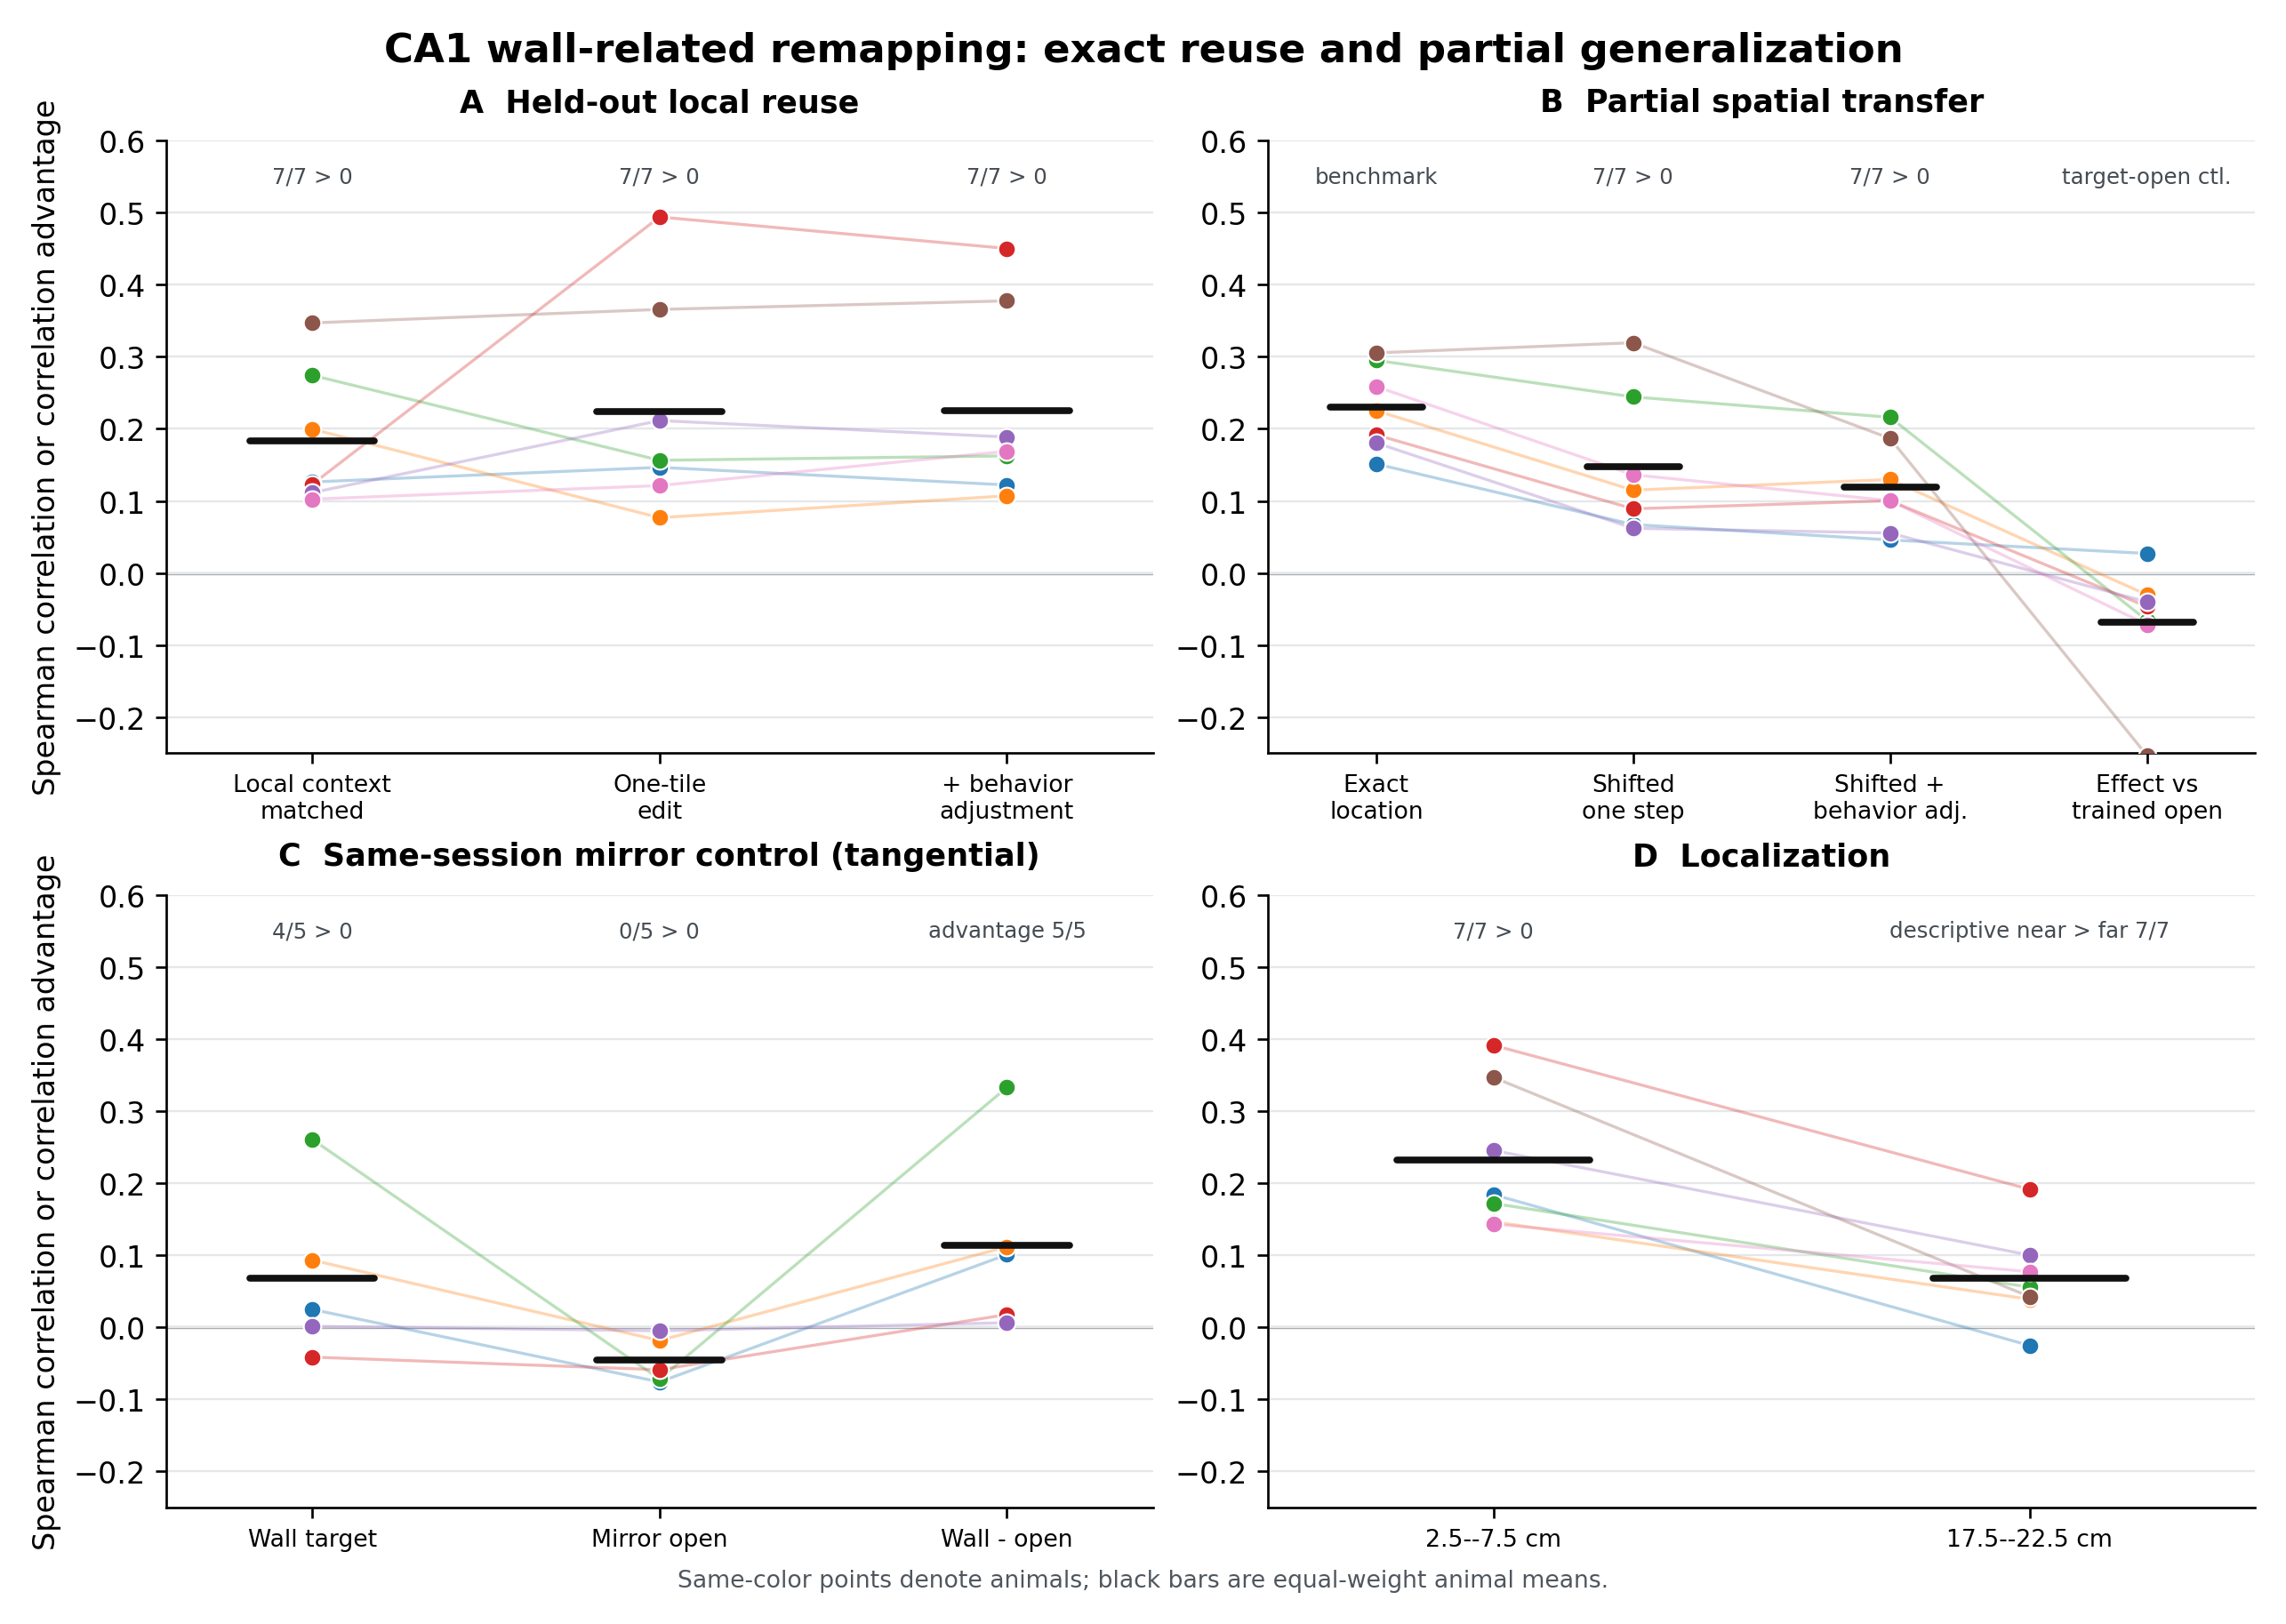
\includegraphics[width=\linewidth]{local_wall_update_transfer.png}
\caption{\textbf{Exact reuse, shifted transfer, and key controls.}
\textbf{A}, wall-minus-open prediction advantages at the same seam, including
the single-tile contrast and its behavior-adjusted estimate.
\textbf{B}, the query-matched exact-location benchmark, the translated
source-effect prediction, its behavior-adjusted estimate, and its specificity
against a training-derived target-open profile.
\textbf{C}, the same-session mirror-open control on its supported paired
subset: correlations for the wall and mirror-open targets and their
wall-minus-open advantage. Only five animals had eligible paired support.
\textbf{D}, descriptive near and far bands for the single-tile test; the bands
were separately eligible and should not be read as a paired estimate. Points
are animal means; bars show the across-animal mean.}
\label{fig:main}
\end{figure}

\subsection{Behavioral and spatial controls define the phenomenon}

Because animals may run differently near internal barriers, we re-estimated
local neural response maps with covariates for speed, first and second circular
harmonics of heading, elapsed time, and spatial sampling. The behavior-adjusted
translated effect remained positive in all seven animals
(\(\meanrho=0.119\)). Its specificity against the training-derived target-open
profile was \(0.172\), and its advantage over a source-open predictor was
\(0.138\), both seven of seven. Omitting elapsed time changed these values by
less than \(0.003\).

We next compared the correctly oriented source with empirical source seams at
the same 25 cm target-midpoint distance but with an incorrect signed wall
normal. This control retains the observed neural maps, registered-cell
identities, target response, and source-target lag while breaking the correct
wall relation. The correct-minus-incorrect advantage was \(0.101\), positive in
all seven animals. Complete enumeration of the \(2^7\) animal-level sign
assignments placed the observed mean in the upper \(1/128\) of that descriptive
null. The result remained positive in every leave-one-animal-out summary.

This pooled comparison does not eliminate spatial continuity. When restricted
to tangential translations with both a 25 cm midpoint distance and a 5 cm
nearest-strip lag, the correct-orientation advantage was only \(0.040\),
positive in three of six animals (sign-flip tail fraction \(0.25\)). Both
correctly and incorrectly oriented tangential sources predicted the target.
Thus the pooled null shows that the full effect is not an arbitrary
equal-midpoint match, but the most tightly distance-matched stratum does not
identify a general orientation-specific rule.

The registered-wall and target-wall strips could nevertheless share generic
nearby place-field structure. We therefore defined a stricter within-session
control before inspecting its neural endpoint in the project workflow. For
each wall target, a mirror-open seam in the same target session was matched for
translation distance, axis, signed normal, relative bins, and registered
cells. The geometry permits this match only for tangential translations.
Although 104 labeled configurations were feasible, paired-support gates
retained 72 triplets in five animals; two animals had no admissible control.

On this restricted subset, the globally demeaned source vector favored the
wall target over the mirror-open target by \(0.114\), positive in all five
eligible animals (Fig.~\ref{fig:main}C). Absolute source-to-wall correlation
was positive in four of five animals (\(\meanrho=0.068\)), and a direct
within-session wall-minus-open difference-vector score was positive in four of
five (\(\meanrho=0.077\)). The raw-rate primary was positive in only three of
five. The exact animal-level sign-flip tail fraction for the demeaned advantage
was \(1/32\), and every leave-one-animal-out mean remained positive. The
strongest justified reading is narrow: the transferred contrast distinguished
a wall target from an equally displaced open location in the supported
demeaned tangential cases. It does not establish the full seven-animal effect,
normal-axis transfer, or raw-rate specificity.

A coherent source-cell identity permutation further showed descriptive
upper-tail fractions below \(0.01\) in five animals and values of \(0.069\) and
\(0.060\) in the other two. Registered-cell correspondence therefore
contributes to the prediction, although the effect is not uniformly strong.
Additional exploratory analyses of direction, composition, experience, and a
former-barrier endpoint are reported in Supplementary
Section~\ref{sec:supplementary} rather
than treated as tests of the central phenomenon.

\begin{table}[t]
\centering
\caption{\textbf{Evidence for partial cross-location generalization.} Values
are means across animal-level estimates. Sign counts are descriptive
consistency summaries.}
\label{tab:evidence}
\small
\begin{tabularx}{\linewidth}{@{}>{\raggedright\arraybackslash}p{0.28\linewidth}
  rr>{\raggedright\arraybackslash}X@{}}
\toprule
Test & Mean & Sign & Supported interpretation\\
\midrule
Context-matched exact seam & \(0.184\) & \(7/7\) &
Local wall-open population contrast recurs across layouts.\\
Single-tile exact seam & \(0.225\) & \(7/7\) &
Exact-location reuse survives a cleaner local counterfactual.\\
Behavior-adjusted single tile & \(0.225\) & \(7/7\) &
Measured speed, heading, time, and sampling do not explain reuse.\\
Shifted source effect & \(0.148\) & \(7/7\) &
A cell-resolved wall contrast predicts a different location.\\
Query-matched exact effect & \(0.230\) & \(7/7\) &
Exact reuse exceeds shifted transfer.\\
Behavior-adjusted shifted effect & \(0.119\) & \(7/7\) &
Measured behavior does not eliminate transfer.\\
Correct minus wrong orientation at 25 cm & \(0.101\) & \(7/7\) &
The pooled effect exceeds an equal-midpoint empirical spatial null.\\
Mirror-open advantage & \(0.114\) & \(5/5\) &
Demeaned tangential subset favors a wall over an equally displaced open seam.\\
\bottomrule
\end{tabularx}
\end{table}

\section{Discussion}

The central result is partial cross-location generalization in a hippocampal
spatial code. A cell-resolved wall-minus-open response estimated from one group
of geometries predicted a later response at the same seam, and a contrast
estimated at a different seam predicted a later target-wall response. The
cross-location prediction was positive in every animal, survived adjustment
for measured behavior, and was weaker than the matched exact-location
prediction. Local boundary-related remapping is therefore neither independent
across coordinates nor fully location invariant.

The finding goes beyond the established observation that boundaries influence
place fields. Boundary-vector models explain how fields can arise from inputs
tuned to distance and direction from boundaries
\citep{HartleyEtAl2000,BarryEtAl2006}, and barrier manipulations have shown
local field formation, duplication, and geometry-dependent remapping
\citep{RivardEtAl2004,LeeEtAl2025}. Those results make some recurrence
plausible. They do not by themselves demonstrate that a signed vector of
responses, indexed by the identities of longitudinally registered CA1 cells,
generalizes from one physical seam to another under held-out evaluation.

The attenuation relative to exact reuse is equally informative. It shows that
the response is not reconstructed independently at every seam, yet that most
predictive structure remains tied to the original location. This intermediate
organization is the empirical result; no latent operator or particular
biological decomposition is required to state it.

Several alternative explanations remain. First, smooth or repeated place
fields can correlate at nearby seams. The non-overlapping strips, square
residuals, target-open specificity, equal-midpoint wrong-orientation null, and
mirror-open control constrain this account. They do not eliminate it: the
fully distance-matched tangential orientation contrast was inconsistent, and
the mirror control was limited to five animals and demeaned tangential
translations. Second, unmeasured
behavior such as attention, wall inspection, acceleration, or route choice
could contribute despite adjustment for measured kinematics. Third, the fixed
environment sequence leaves environment-specific order confounded with the
single-tile contrast. Fourth, registration and activity thresholds select
cells stable enough to be observed across sessions. Fifth, the identity
permutation is not an ideal exchangeability test for correlated place-cell
populations.

Exploratory analyses of composition, experience, and a former-barrier endpoint
were either underpowered or unstable and are reported separately in the
Appendix. They do not alter the positive cross-location result and should not
be interpreted as broad tests of hippocampal composition, learning, or
innateness.

The decisive next experiment is compact. Use a symmetric lattice arena with
four equivalent candidate wall seams. Randomly assign source and target
locations, wall orientation, insertion or removal, and session order within
animal. Estimate a source wall-open contrast, then test exact reuse, translated
reuse, and a distance-matched open target in the same later session. This
design would distinguish wall-specific generalization from smooth spatial
deformation while removing the fixed-order confound.
The present effect sizes provide realistic targets: an exact-location
correlation near \(0.23\), shifted correlation near \(0.12\)--\(0.15\), and a
shifted-minus-exact penalty near \(0.08\).

\section{Materials and methods}

\subsection{Dataset and analysis cohort}

We reanalysed the public longitudinal dorsal-CA1 calcium-imaging dataset of
\citet{LeeEtAl2025,LeeKeinathBrandon2024Dataset}. The tracked analysis cohort contains seven
mice, 5,413 neurons, 207 sessions, a familiar outer square, and nine
internal-wall geometries arranged on a common lattice. Cell identities were
registered across sessions in the source dataset. The original study describes
surgery, imaging, behavior, preprocessing, registration, and animal procedures.
No new animal experiments were performed.

\subsection{Spatial representation and oriented seams}

The arena was expressed in a common allocentric coordinate system. A candidate
internal-wall location was represented as an oriented seam \(s=(p\rightarrow
q)\) between adjacent lattice tiles, with a signed normal from tile \(p\) to
tile \(q\). The binary state \(z_{e,s}\) indicated whether environment \(e\)
blocked that adjacency. Local strips were partitioned into 5 cm spatial bins
at defined distances from the seam. Analyses used only bins and registered
cells satisfying the relevant occupancy, activity, and common-support gates.
Source and target strips in the cross-location analysis shared no 5 cm bin.

\subsection{Local response vectors and square residuals}

Let \(r_{i,e,s}\) denote the local response estimate for registered cell \(i\)
in environment \(e\) at seam \(s\), averaged over eligible spatial bins after
the analysis-specific preprocessing. The corresponding bracketing-square
estimate was \(r_{i,\square(e),s}\). The primary environment-specific response
was
\[
  \delta_{i,e,s}=r_{i,e,s}-r_{i,\square(e),s}.
\]
For globally demeaned variants, each vector's common-cell mean was removed
before correlation. This suppresses population-wide rate shifts and makes the
score depend on relative cell identities.

\subsection{Training profiles and held-out scoring}

For a target query \((e^\ast,s^\ast)\), training environments were selected
without using the neural response of \(e^\ast\). At a source seam \(s\), the
wall and open profiles were
\[
 \boldsymbol{\mu}_{W,s}
   = \operatorname{mean}_{e\in\mathcal T:z_{e,s}=1}
     \boldsymbol{\delta}_{e,s},
 \qquad
 \boldsymbol{\mu}_{O,s}
   = \operatorname{mean}_{e\in\mathcal T:z_{e,s}=0}
     \boldsymbol{\delta}_{e,s},
\]
computed on the common registered-cell support. The estimated source effect was
\(\mathbf d_s=\boldsymbol{\mu}_{W,s}-\boldsymbol{\mu}_{O,s}\).
The held-out outcome was \(\boldsymbol{\delta}_{e^\ast,s^\ast}\).
Scores were Spearman correlations across registered cells. Wall-open
advantages compare correlations within the same query and cell support.

The exact-location estimator set \(s=s^\ast\). Its context-matched version
restricted training comparisons so the broader internal-wall context was
balanced between the wall and open profiles. The reported exact-location
benchmark for shifted transfer was recomputed on the exact queries, sessions,
cells, and local supports eligible for the shifted analysis.

\subsection{Single-tile counterfactual}

The \(u\) and \(o\) geometries differed at one lattice tile: \(u\) blocked
tiles \(\{4,5\}\), whereas \(o\) blocked only tile \(\{4\}\). We formed the
cell-wise \(u-o\) contrast at the focal seam and evaluated wall and open
outcomes at that seam in held-out \(i\), \(l\), and \(t\) geometries. Near
(2.5--7.5 cm) and far (17.5--22.5 cm) bands were screened separately, so their
difference is descriptive. For the order-placebo analysis, we formed
later-minus-earlier contrasts at unchanged seams with the same processing and
compared their signs with the actual \(u-o\) contrast.

\subsection{Cross-location transfer}

For each eligible target seam, the source seam was a non-overlapping lattice
seam 25 cm away with the same signed wall normal and admissible wall/open
training support. Source training and target outcome sessions were disjoint.
The primary shifted score was
\[
  \rho_{\mathrm{shift}}
  =\rho_{\mathrm S}
    \left(\mathbf d_{s_{\mathrm{source}}},
    \boldsymbol{\delta}_{e^\ast,s_{\mathrm{target}}}\right).
\]
Secondary specificity scores compared the source effect with a
training-derived open profile at the target and compared source-wall with
source-open predictors. The exact-location benchmark used
\(\mathbf d_{s_{\mathrm{target}}}\) on the identical held-out query support.
Stored-map and behavior-adjusted audits agreed on 405 target queries and 658
source pairs, including their session and seam identities and their counts of
common cells and bins. That audit did not hash the complete cell-ID or
bin-coordinate arrays.

\subsection{Behavior-adjusted response estimates}

We estimated activity jointly with spatial-bin indicators and nuisance
covariates for instantaneous speed, sine and cosine of heading, second heading
harmonics, and elapsed time. Spatial effects were evaluated at a common
reference covariate distribution calibrated from the first familiar-square
session. The no-time sensitivity omitted elapsed time but retained the other
covariates. Target-session activity was used to estimate nuisance coefficients
for that target map, but target neural outcomes never entered source-profile
training.

\subsection{Same-session mirror-open control}

Before inspecting the neural endpoint within the project workflow, we defined
a mirror-open seam in the same target session as each target wall. It matched
the source-wall pair in translation distance, translation axis, signed normal,
relative spatial bins, and registered cells. Both source-to-target nearest-bin
distances were 5 cm. Only tangential translations admitted this exact
geometric pairing. Primary scoring used globally demeaned source and target
vectors. Eligibility required a complete source, wall-target, and open-target
triplet on common support.

\subsection{Spatial-null calibration}

We calibrated two empirical spatial controls at the animal level. The first
compared correctly oriented source seams with incorrectly oriented sources at
the same 25 cm target-midpoint distance. A tangential stratum additionally
matched translation axis and the 5 cm nearest-strip lag. The second compared
the wall target with the same-session reflected-open target described above.
Both controls retain the observed neural maps and therefore their place-field
smoothness. For each paired animal-level contrast, we enumerated all \(2^N\)
sign assignments and calculated the fraction of null means at least as large
as the observed mean. These are descriptive exact sign-flip calibrations, not
confirmatory population \(p\)-values.

\subsection{Cell-identity permutation}

For each animal, we generated 999 coherent random mappings of source-cell
identities while preserving query geometry, target vectors, support sizes, and
the mapping across all queries in that permutation. The descriptive upper-tail
fraction was \((1+n_{\mathrm{null}\geq\mathrm{observed}})/(1000)\). Correlations
and registration constraints limit exchangeability; the fractions were used
as identity-specificity diagnostics rather than inferential population
\(p\)-values.

\subsection{Direction, composition, and experience analyses}

Direction controls compared eligible source-target pairs with same or opposite
signed wall normals while documenting translation axis, distance, overlap, and
layout matching. No single comparison simultaneously matched all of these
features across the full cohort.

For composition, we identified complete wall-state factorials in which two
single-wall effects and their joint state could be estimated. The additive
prediction was the sum of the two single effects. It was compared with an
oracle best-single-component predictor using correlation and normalized
prediction error. Only two repetitive factorials and five eligible animals
were available.

Experience analyses contrasted transfer changes across exposure blocks using
difference-in-differences variants. Because geometry, order, and exposure were
not independently randomized, these estimates were treated as exploratory
sensitivity analyses and not as evidence for learning.

\subsection{Independent former-barrier analysis}

We used the public neutral-barrier data from \citet{BlairEtAl2023}
to test whether the former barrier center retained an excess neural similarity
relative to matched control locations after removal. The primary endpoint was
a Pearson correlation among active cells, averaged as a former-barrier
center-minus-control contrast. Its definition was written before the neural
endpoint was run in the local project workflow. Spearman scoring and
leave-one-animal-out summaries were sensitivities.

\subsection{Statistical reporting and reproducibility}

Animals were treated as the biological units. We report animal-level means,
sign counts, query counts, and explicitly labeled descriptive permutation
fractions. No cell-level or query-level observation was presented as an
independent animal replicate. The analyses are exploratory: neither the
original experiment nor the present reanalysis was preregistered for the
cross-location hypothesis.

All figure values derive from tracked machine-readable source files. The
repository contains scripts, eligibility ledgers, result summaries, design
locks, and an inspectable Git history. The principal manuscript figure is
generated from its tracked source-data CSV.

\section{Supplementary exploratory analyses}
\label{sec:supplementary}

\subsection{Direction and two-wall composition}

Direction controls did not identify a general orientation rule. Same- versus
opposite-signed normals for tangential translation favored the same direction
in three of six eligible animals. A normal-axis comparison against
opposite-facing or overlapping alternatives was positive in four of seven. A
less controlled same- versus opposite-away comparison was positive in all
seven, but it also changed strip distance and layout. These analyses support
transfer between selected corresponding seams, not rotation- or
direction-invariant transport.

Only two complete two-wall factorials were available, both involving the same
bit and donut layouts. In five eligible animals, the demeaned additive
predictor reached mean correlation \(0.153\), below an oracle
best-single-component predictor at \(0.178\). The additive advantage was
\(-0.024\) and positive in one of five animals. This sparse support provides no
positive evidence for linear two-wall composition but cannot establish general
non-compositionality.

\subsection{Experience and former-barrier endpoints}

A transfer-by-experience difference-in-differences estimate was positive under
one stored-map specification (mean \(0.045\), four of four eligible animals),
but raw-rate and stricter sensitivity analyses were unstable. Environment
order, exposure number, and geometry were not independently varied, so the
data do not identify experience-dependent stabilization or innateness.

In an independent neutral-barrier dataset \citep{BlairEtAl2023}, the locked
Pearson-active former-barrier center-minus-control endpoint was negative in all
leave-one-animal-out summaries (animal mean \(-0.183\); one of six animals
positive). A Spearman sensitivity was near zero (mean \(0.001\); three of six
positive). We therefore found no evidence for a persistent local
representational scar under that endpoint.

\section*{Data and code availability}

The CA1 source data are available through the archive cited by
\citet{LeeKeinathBrandon2024Dataset}. The independent miniscope data are available through
the archive cited by \citet{BlairData2023}. Analysis code, derived source
tables, audit reports, and manuscript sources are publicly available at
\url{https://github.com/asim-v/ca1-wall-update-transfer}. The public release
excludes the original raw recordings, which remain available from their source
archives.

\section*{Acknowledgments}

We thank the authors of the source studies for making their longitudinal
datasets available.

\section*{Author contributions}

J.E.B.S. conceived the study, developed and performed the analyses, interpreted
the results, prepared the visualizations, and wrote the manuscript.

\section*{Competing interests}

The author declares no competing interests.

\bibliographystyle{plainnat}
\bibliography{references}

\end{document}
